%==============================================================================
% Sjabloon poster bachproef
%==============================================================================
% Gebaseerd op document class `a0poster' door Gerlinde Kettl en Matthias Weiser
% Aangepast voor gebruik aan HOGENT door Jens Buysse en Bert Van Vreckem

\documentclass[a0,portrait]{hogent-poster}

% Info over de opleiding
\course{Bachelorproef}
\studyprogramme{toegepaste informatica}
\academicyear{2022-2023}
\institution{Hogeschool Gent, Valentin Vaerwyckweg 1, 9000 Gent}

% Info over de bachelorproef
\title{Criteria waarop native applicaties ontwikkelen interessanter wordt dan 
het ontwikkelen van cross-platform applicaties}
%\subtitle{Ondertitel (eventueel)}
\author{Jonathan De Catelle}
\email{jonathan.decatelle@student.hogent.be}
\supervisor{Gilles Blondeel}
\cosupervisor{Arno Boel (Delaware)}

% Indien ingevuld, wordt deze informatie toegevoegd aan het einde van de
% abstract. Zet in commentaar als je dit niet wilt. 
\specialisation{Mobile \& Enterprise developer}
\keywords{Mobiele applicatieontwikkeling, Kotlin, Android Studio, React native, Cross-platform, Native}
\projectrepo{https://github.com/JonathanDeCatelle/DeCatelleJonathan-BP-latex}

\begin{document}

\maketitle

\begin{abstract}
De keuze tussen cross-platform en native ontwikkeling is cruciaal bij het ontwikkelen 
van mobiele apps. Deze studie vergelijkt ontwikkeltijden, prestaties en schaalbaarheid 
van verschillende functionaliteiten tussen beide methoden. Resultaten tonen aan dat 
native ontwikkeling betere prestaties heeft voor basisfunctionaliteiten en audio-/videospelers, 
vergelijkbare prestaties bij het gebruik van sensoren, en een groot verschil in 
notificatiecreatie tussen Android en React Native, waarbij Android beter presteert. 
Het onderzoek biedt inzicht voor ontwikkelaars om een weloverwogen keuze te maken bij 
het kiezen van de ontwikkelmethode.
\end{abstract}

\begin{multicols}{2} % This is how many columns your poster will be broken into, a portrait poster is generally split into 2 columns

\section{Introductie}
Bij het ontwikkelen van mobiele applicaties is de keuze tussen native en cross-platform 
ontwikkeling van groot belang. Deze keuze wordt beïnvloed door factoren zoals tijd, budget, 
performantie, schaalbaarheid en functionaliteiten. 

Dit onderzoek vergelijkt de ontwikkeltijden, prestaties en schaalbaarheid van 
functionaliteiten tussen native en cross-platform 
ontwikkeling. Het doel is om inzicht te bieden aan ontwikkelaars en andere belanghebbenden, 
zodat zij een weloverwogen beslissing kunnen nemen bij het kiezen van de ontwikkelmethode.

Het onderzoek richt zich op individuele functionaliteiten en wordt uitgevoerd op één 
platform om de focus te behouden tot native en cross-platform, niet de platformen zelf. 

De conclusies en antwoorden op de 
onderzoeksvragen zullen helpen bij het maken van keuzes en het begrijpen 
van de ontwikkeltijd, performantie en schaalbaarheid van functionaliteiten.

\section{Onderzoek}
Om de functionaliteiten van native en cross-platform applicaties te testen en 
te vergelijken wordt er gekeken naar de ontwikkeltijd, performantie en schaalbaarheid.

Voor het meten van de ontwikkeltijd wordt gekeken naar de tijd die nodig is om elke 
functionaliteit te implementeren, alsook eventuele bugs of problemen, wordt gedocumenteerd.

De performantie van zowel de native als de cross-platform applicaties wordt gemeten 
met behulp van de Android profiler in Android Studio en de Firebase Performance
Monitoring tool. Op die manier kan de performantie van beide applicaties eerlijk worden vergeleken 
omdat er geen platform specifieke tools worden gebruikt.

\begin{center}
  \captionsetup{type=figure}
  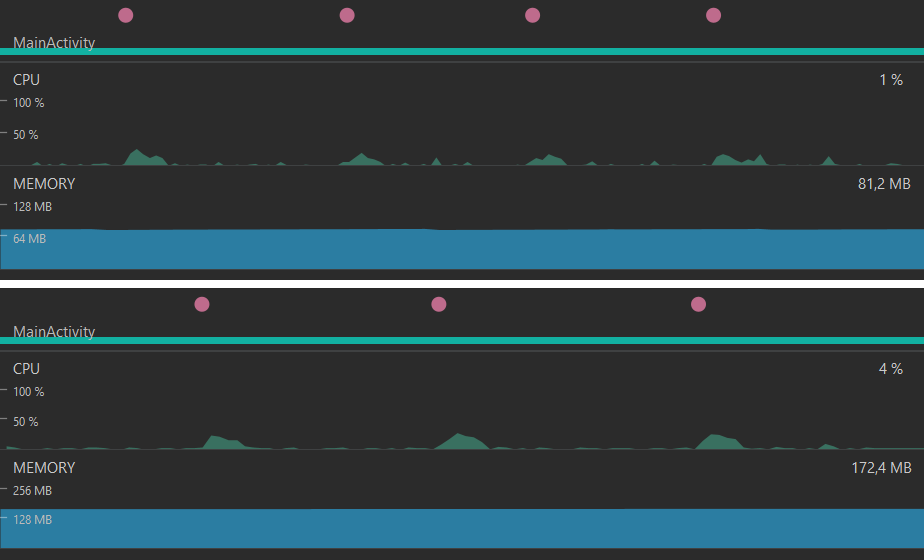
\includegraphics[width=1.0\linewidth]{notificaties1.png}
  \captionof{figure}{Overzicht CPU en geheugen gebruik tijdens aanmaken notificaties bij Android(bovenste schermafbeelding) en React Native(onderste schermafbeelding).}
\end{center}

\begin{center}
  \captionsetup{type=figure}
  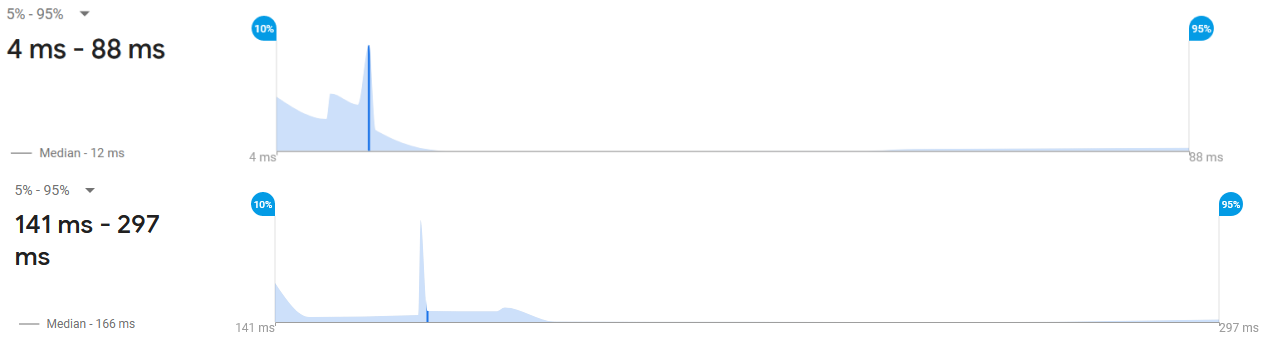
\includegraphics[width=1.0\linewidth]{notificaties2.png}
  \captionof{figure}{Overzicht tijdsduur aanmaken notificaties bij Android(bovenste schermafbeelding) en React Native(onderste schermafbeelding).}
\end{center}

Om de schaalbaarheid van de applicaties en libraries te testen wordt de complexiteit van
de code geanalyseerd en wordt er gekeken naar de mogelijkheid om de code op te delen in
herbruikbare componenten. Dit bevordert de schaalbaarheid van de applicatie.

Door deze factoren te testen, kan een gedetailleerde vergelijking worden gemaakt tussen 
native en cross-platform applicaties.

\section{Conclusies}
De ontwikkeltijd bij cross-platform is over het algemeen langer vanwege de extra 
installatie van libraries en de noodzaak om meer code te schrijven voor dezelfde 
functionaliteit. De compiletijd is ook langer bij cross-platform, maar de hot 
reload-functie van React Native compenseert dit en bespaart tijd tijdens het ontwikkelen. 

Qua performantie is er een groot verschil bij het aanmaken van notificaties, waarbij 
cross-platform veel langer duurt. Daarnaast zijn de verschillen in tijdsduur, 
CPU-gebruik en geheugengebruik wel merkbaar vanuit de resultaten maar niet storend 
voor de gebruiker. Het geheugengebruik is echter gemiddeld 2,5 keer hoger bij 
cross-platform vanwege de extra libraries. Wat betreft schaalbaarheid zijn zowel 
native als cross-platform methoden vergelijkbaar in complexiteit en hebben ze een 
hoge herbruikbaarheid van code. 

Uit het onderzoek is ook gebleken dat er geen functionaliteiten zijn die cross-platform 
niet ondersteunt en dat alle geïmplementeerde functionaliteiten bruikbaar waren, ondanks de 
verschillen in performantie tussen native en cross-platform.

\section{Toekomstig onderzoek}
Dit onderzoek toont aan dat er een duidelijk verschil is in performantie tussen native en 
cross-platform frameworks. Dit roept de vraag op of dit verschil bij alle functionaliteiten 
aanwezig zal zijn, en of er zelfs functionaliteiten zijn die beter presteren bij cross-platform. 

Verder onderzoek kan worden uitgebreid naar andere cross-platform frameworks zoals Flutter of 
.NET MAUI om te zien of deze betere prestaties leveren zonder in te boeten op ontwikkeltijd en 
schaalbaarheid. Ook kan het onderzoek worden uitgebreid naar andere native frameworks zoals 
Java of andere native platformen zoals iOS. Het debat over native versus cross-platform zal 
altijd blijven bestaan, aangezien er voortdurend nieuwe frameworks en technologieën opduiken. 

Hoewel er geen definitief antwoord is op welke ontwikkelingsmethode/framework uiteindelijk 
de beste is, kunnen dergelijke onderzoeken ontwikkelaars helpen om weloverwogen keuzes te 
maken bij het selecteren van een technologie voor hun specifieke project.

\end{multicols}
\end{document}